\documentclass[aspectratio=169, border=0.2cm, xcolor=table]{beamer}

\usetheme{ccc}

\usepackage{fontspec}
\usepackage{blindtext}
\usepackage{graphicx}
\usepackage{listings}
\usepackage{tikz}
\usepackage{pgfplots}
\usepackage{pgf-pie}
\usepackage{pifont}
\usepackage{booktabs}
\usepackage{changepage}
\usepackage{amsmath}
\usetikzlibrary{positioning}
\usetikzlibrary{arrows.meta}
\usetikzlibrary{shapes.geometric}
\usetikzlibrary{calc}
\usetikzlibrary{fit}
\usetikzlibrary{graphs}
\usetikzlibrary{matrix}
\usetikzlibrary{backgrounds}

\definecolor{lightgray}{gray}{0.9}

% bright paul tol's colors
\definecolor{bBlue}{HTML}{4477AA}
\definecolor{bCyan}{HTML}{66CCEE}
\definecolor{bGreen}{HTML}{228833}
\definecolor{bYellow}{HTML}{CCBB44}
\definecolor{bRed}{HTML}{EE6677}
\definecolor{bPurple}{HTML}{AA3377}
\definecolor{bGray}{HTML}{BBBBBB}

% vibrant paul tol's colors
\definecolor{vBlue}{HTML}{0077BB}
\definecolor{vCyan}{HTML}{33BBEE}
\definecolor{vTeal}{HTML}{009988}
\definecolor{vOrange}{HTML}{EE7733}
\definecolor{vRed}{HTML}{CC3311}
\definecolor{vMagenta}{HTML}{EE3377}
\definecolor{vGray}{HTML}{BBBBBB}

% muted paul tol's colors
\definecolor{mIndigo}{HTML}{332288}
\definecolor{mCyan}{HTML}{88CCEE}
\definecolor{mTeal}{HTML}{44AA99}
\definecolor{mGreen}{HTML}{117733}
\definecolor{mOlive}{HTML}{999933}
\definecolor{mSand}{HTML}{DDCC77}
\definecolor{mRose}{HTML}{CC6677}
\definecolor{mWine}{HTML}{882255}
\definecolor{mPurple}{HTML}{AA4499}

% pale paul tol's colors
\definecolor{pBlue}{HTML}{BBCCEE}
\definecolor{pCyan}{HTML}{CCEEFF}
\definecolor{pGreen}{HTML}{CCDDAA}
\definecolor{pYellow}{HTML}{EEEEBB}
\definecolor{pRed}{HTML}{FFCCCC}
\definecolor{pGray}{HTML}{DDDDDD}

% dark paul tol's colors
\definecolor{dBlue}{HTML}{222255}
\definecolor{dCyan}{HTML}{225555}
\definecolor{dGreen}{HTML}{225522}
\definecolor{dYellow}{HTML}{666633}
\definecolor{dRed}{HTML}{663333}
\definecolor{dGray}{HTML}{555555}

% light paul tol's colors
\definecolor{lBlue}{HTML}{77AADD}
\definecolor{lCyan}{HTML}{99DDFF}
\definecolor{lMint}{HTML}{44BB99}
\definecolor{lPear}{HTML}{BBCC33}
\definecolor{lOlive}{HTML}{AAAA00}
\definecolor{lYellow}{HTML}{EEDD88}
\definecolor{lOrange}{HTML}{EE8866}
\definecolor{lPink}{HTML}{FFAABB}
\definecolor{lGray}{HTML}{DDDDDD}

\tikzset{
  onslide/.code args={<#1>#2}{%
    \only<#1>{\pgfkeysalso{#2}}% \pgfkeysalso doesn't change the path
  },
  temporal/.code args={<#1>#2#3#4}{%
    \temporal<#1>{\pgfkeysalso{#2}}{\pgfkeysalso{#3}}{\pgfkeysalso{#4}}%
  },
  hidden/.style = {opacity=0},
  uncover/.style = {temporal=#1{hidden}{}{hidden}},
  drawalert/.style = {temporal=#1{}{color=alerted text.fg}{}}
}

\begin{document}
\begin{frame}
\end{frame}
\begin{frame}\frametitle{Scratch}
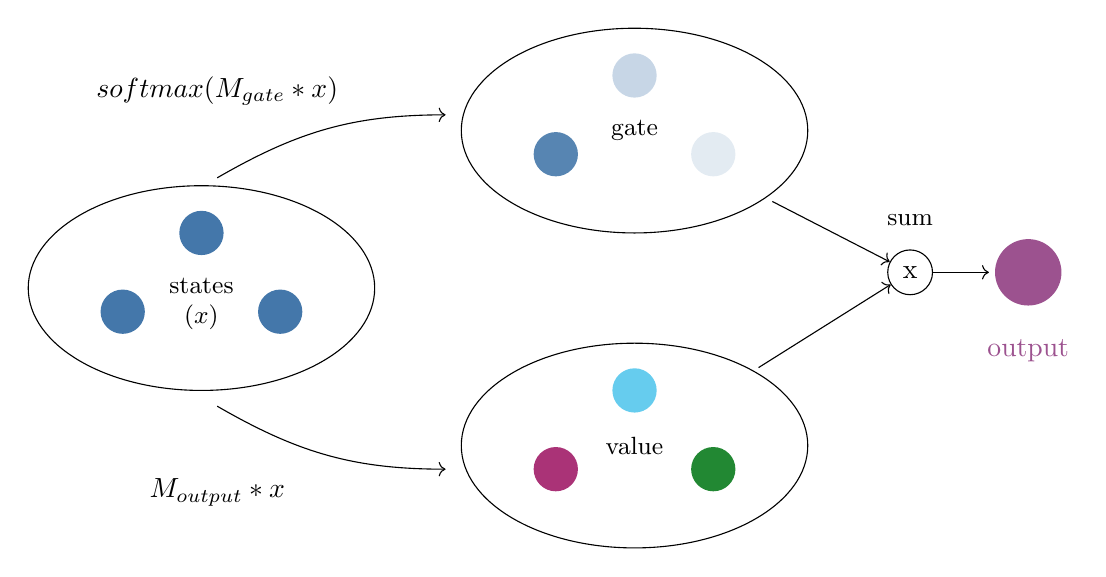
\begin{tikzpicture}
  \begin{scope}[local bounding box=init]
    \fill[color=bBlue, radius=0.8em]
    (0,0) circle[]
    (1,1) circle[]
    (2,0) circle[]
    ;
    \draw (1,0.3) ellipse[x radius=2.2cm, y radius=1.3cm] +(0,-0.2) node[font=\small,align=center] {states \\ $(x)$};
  \end{scope}

  \begin{scope}[xshift=5.5cm, yshift=-2cm]
    \fill[color=bPurple, radius=0.8em] (0,0) circle[];
    \fill[color=bCyan, radius=0.8em] (1,1) circle[];
    \fill[color=bGreen, radius=0.8em] (2,0) circle[];
    \draw (1,0.3) ellipse[x radius=2.2cm, y radius=1.3cm] node[font=\small] (value) {value};
  \end{scope}


  \begin{scope}[xshift=5.5cm, yshift=2cm]
    \fill[color=bBlue!90, radius=0.8em] (0,0) circle[];
    \fill[color=bBlue!30, radius=0.8em] (1,1) circle[];
    \fill[color=bBlue!15, radius=0.8em] (2,0) circle[];
    \draw (1,0.3) ellipse[x radius=2.2cm, y radius=1.3cm] node[font=\small] (gate) {gate};
  \end{scope}

  \fill[color=bPurple!80!bCyan] (11.5,0.5) circle[radius=1.2em] +(0,-1) node (out) {output};

  \node[draw,circle] (mult) at (10,0.5) {x};

  \draw (mult) edge[->] (11,0.5);
  \draw ($(gate)!.5!(mult)$) edge[->] (mult);
  \draw ($(value)!.45!(mult)$) edge[->] (mult);
  \draw (1.2, 1.7) edge[out=30, in=180, ->] (4.1, 2.5) node[above=0.8cm]{$softmax(M_{gate} * x)$};
  \draw (1.2, -1.2) edge[out=-30, in=180, ->] (4.1, -2) node[below=0.8cm]{$M_{output} * x$};

  ¸\node[above=0.5em of mult, font=\small] {sum};

\end{tikzpicture}
%%% Local Variables:
%%% TeX-master: "../scratch.tex"
%%% End:

\end{frame}
\end{document}
